\documentclass[border=12pt]{standalone}
\usepackage{tikz}
\usetikzlibrary{positioning, calc, fit, backgrounds, arrows.meta, shapes.multipart}

\definecolor{input}{HTML}{FCE0E1} % salmon
\definecolor{encoder}{HTML}{BFE8C7} % light green
\definecolor{flatten}{HTML}{F2F4C1} % light yellow
\definecolor{perspective_output}{HTML}{FFE2BB} % light orange
\definecolor{fusion}{HTML}{C7B8FF} % purple
\definecolor{trunk}{HTML}{B4D4FF} % light blue
\definecolor{output_head}{HTML}{BFE8C7} % light green

\begin{document}

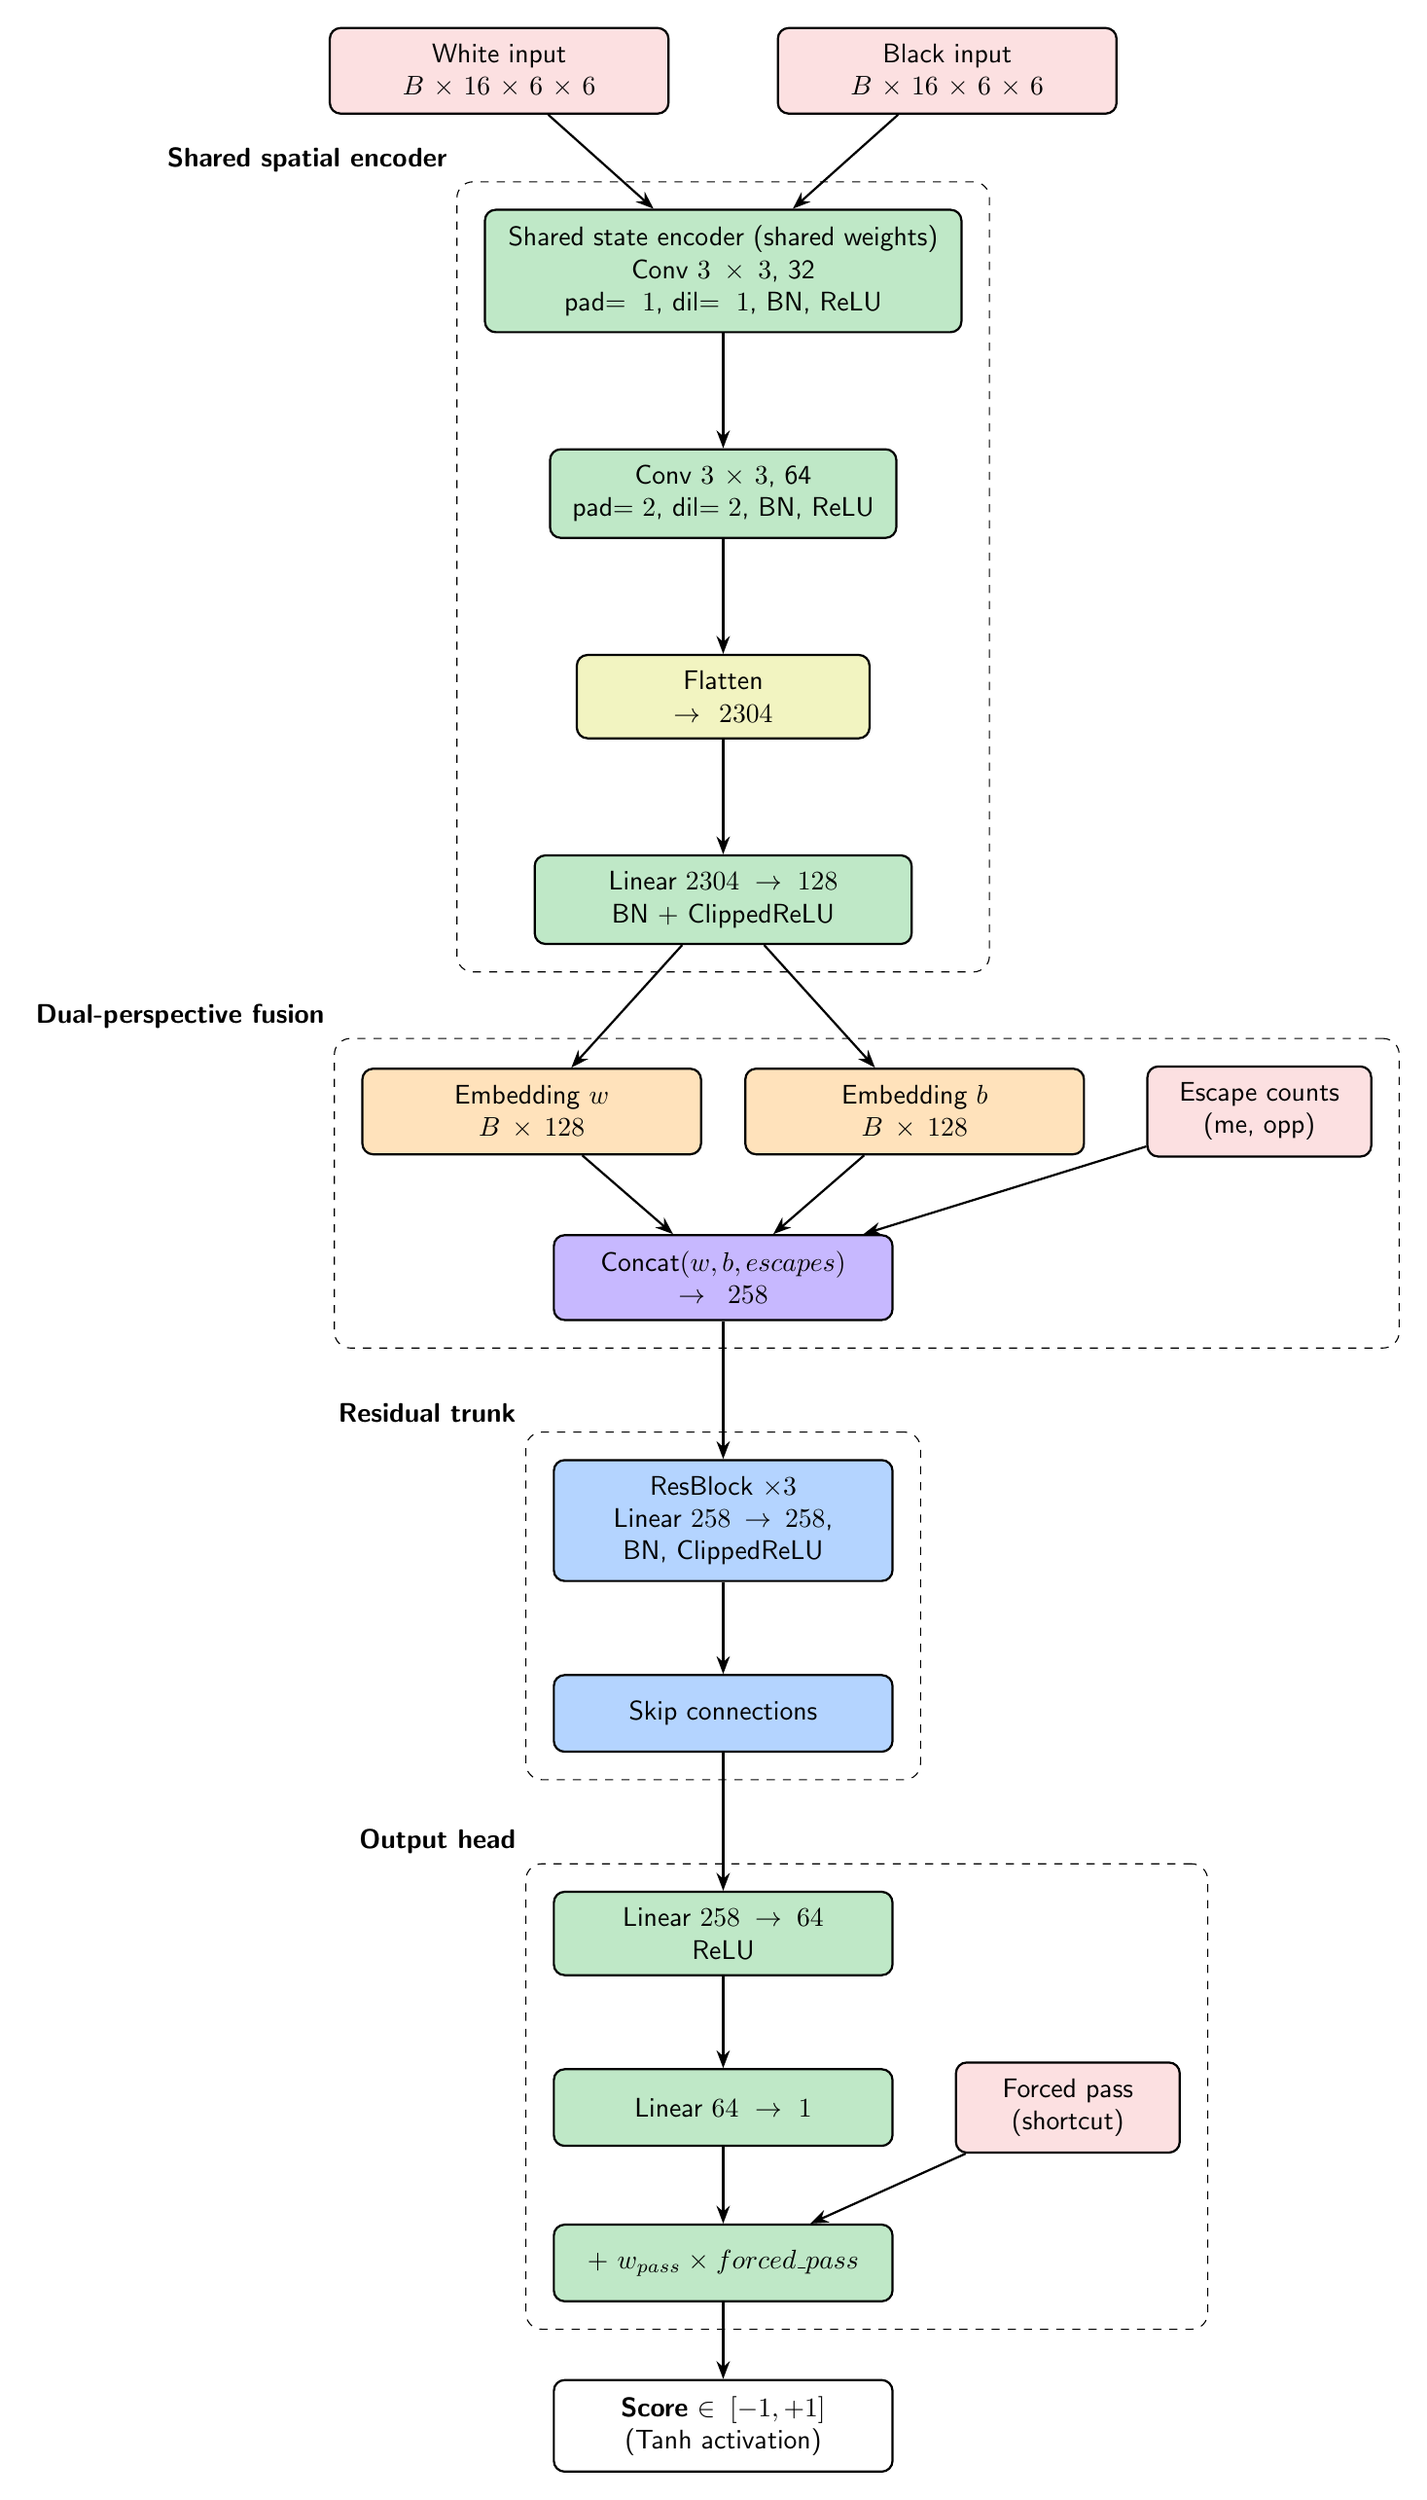
\begin{tikzpicture}[
    >=Stealth,
    thick,
    font=\sffamily,
    node distance=1cm and 1.4cm,
    block/.style={
        draw,
        rounded corners=4pt,
        align=center,
        minimum height=1cm,
        text width=4cm,
        inner sep=6pt
    },
    input/.style={block, fill=input},
    encoder/.style={block, fill=encoder},
    flatten/.style={block, fill=flatten},
    perspective_output/.style={block, fill=perspective_output},
    fusion/.style={block, fill=fusion},
    trunk/.style={block, fill=trunk},
    output_head/.style={block, fill=output_head},
    output/.style={block, fill=none},
    groupbox/.style={
        draw,
        rounded corners=6pt,
        dashed,
        inner sep=10pt,
        label={[font=\bfseries\sffamily]north west:#1}
    }
]

% Inputs
\node[input] (AI) {White input\\$B \times 16 \times 6 \times 6$};
\node[input, right=of AI] (BI) {Black input\\$B \times 16 \times 6 \times 6$};

% Encoder block
\node[encoder, below=1.8cm of $(AI)!0.5!(BI)$, text width=5.8cm] (E1) {Shared state encoder (shared weights)\\Conv $3\times 3$, 32\\pad$=1$, dil$=1$, BN, ReLU};
\node[encoder, below=1.5cm of E1, text width=4.1cm] (E2) {Conv $3\times 3$, 64\\pad$=2$, dil$=2$, BN, ReLU};
\node[flatten, below=1.5cm of E2, text width=3.4cm] (F1) {Flatten\\$\to 2304$};
\node[encoder, below=1.5cm of F1, text width=4.5cm] (Emb) {Linear $2304\to128$\\BN + ClippedReLU};

% Fusion and embeddings
\node[perspective_output, below=1.6cm of Emb, xshift=-2.5cm] (W) {Embedding $w$\\$B \times 128$};
\node[perspective_output, below=1.6cm of Emb, xshift=2.5cm] (B) {Embedding $b$\\$B \times 128$};
\node[input, right=0.8cm of B, text width=2.5cm] (Esc) {Escape counts\\(me, opp)};
\node[fusion, below=1.6cm of $(W)!0.5!(B)$] (C2) {Concat$(w,b,escapes)$\\$\to 258$};

% Residual trunk
\node[trunk, below=1.8cm of C2] (R1) {ResBlock $\times3$\\Linear $258\to258$, BN, ClippedReLU};
\node[trunk, below=1.2cm of R1] (Skip) {Skip connections};

% Output head
\node[output_head, below=1.8cm of Skip] (O1) {Linear $258\to64$\\ReLU};
\node[output_head, below=1.2cm of O1] (O2) {Linear $64\to1$};
\node[input, right=0.8cm of O2, text width=2.5cm] (FP) {Forced pass\\(shortcut)};
\node[output_head, below=1.0cm of O2] (Add) {+ $w_{pass} \times forced\_pass$};
\node[output, below=1.0cm of Add] (Score) {\textbf{Score $\in [-1,+1]$}\\(Tanh activation)};

% Edges
\draw[->] (AI) -- (E1);
\draw[->] (BI) -- (E1);
\draw[->] (E1) -- (E2);
\draw[->] (E2) -- (F1);
\draw[->] (F1) -- (Emb);

\draw[->] (Emb) -- (W);
\draw[->] (Emb) -- (B);
\draw[->] (W) -- (C2);
\draw[->] (B) -- (C2);
\draw[->] (Esc) -- (C2);

\draw[->] (C2) -- (R1);
\draw[->] (R1) -- (Skip);

\draw[->] (Skip) -- (O1);
\draw[->] (O1) -- (O2);
\draw[->] (O2) -- (Add);
\draw[->] (FP) -- (Add);
\draw[->] (Add) -- (Score);

% Boxes
\begin{scope}[on background layer]
    \node[groupbox=Shared spatial encoder, fit=(E1)(E2)(F1)(Emb)] {};
    \node[groupbox=Dual-perspective fusion, fit=(W)(B)(Esc)(C2)] {};
    \node[groupbox=Residual trunk, fit=(R1)(Skip)] {};
    \node[groupbox=Output head, fit=(O1)(O2)(FP)(Add)] {};
\end{scope}

\end{tikzpicture}

\end{document}